% !TeX root = FutureWork.tex
\documentclass[../Dissertation.tex]{subfiles}

\begin{document}

\section{Future Work}

\subsection{Identifying Cycles}
In the current version of the application, cycles within Petri nets are only identifiable by observation. There is no implemented system for highlighting cycles once they are generated. This can become a concern following several iterations of composition. For example, consider the Petri net depicted in Figure \ref{fig:cycle}. This Petri net is created by means of three iterations of composition, and contains a cycle. After only three iterations, the presence of cycles is obscured.

\begin{figure}[H]
\begin{center}
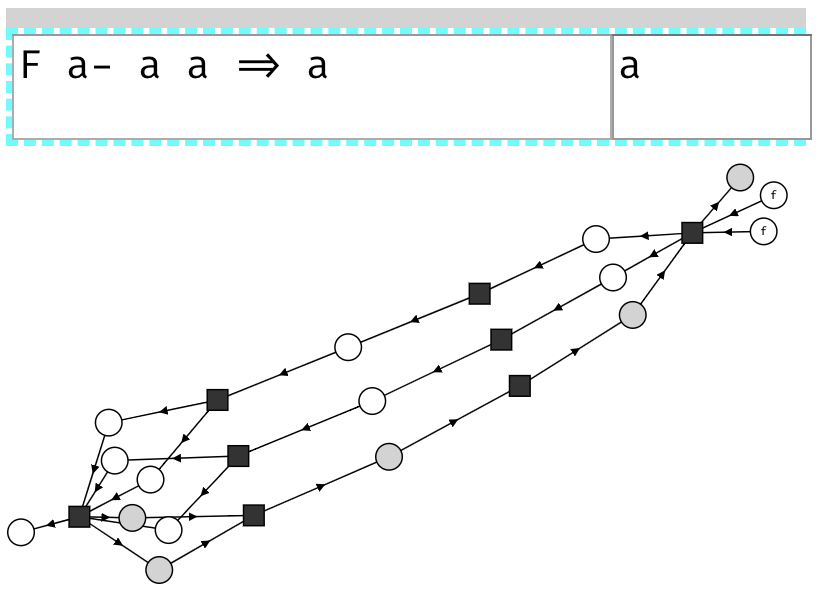
\includegraphics[scale=0.45]{cycle}
\end{center}
\caption{Composite Petri net with a cycle.}
\label{fig:cycle}
\end{figure}

This problem may be resolved by changing the colour of edges which comprise a cycle. Indeed, this approach was used in Figure \ref{fig:petricycle}. However, there remains a broader issue of the increasing complexity of Petri nets after each composition.

\subsection{Petri net Contraction}
Each iteration of composition, within the application, yields a graph with a greater number of nodes. This has the potential to rapidly generate complex graphs which are difficult to analyse. An example of this problem is illustrated in Figure \ref{fig:large}, which presents a Petri net created by six iterations of composition.

\begin{figure}[H]
\begin{center}
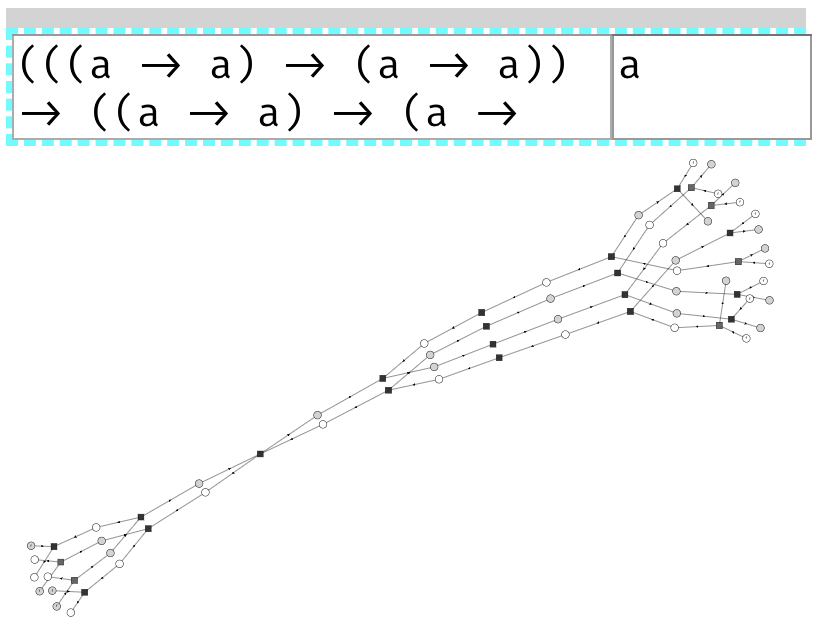
\includegraphics[scale=0.45]{large}
\end{center}
\caption{Composite Petri net generated by six iterations of composition.}
\label{fig:large}
\end{figure}

This complication arises as a consequence of maintaining the composition boundaries. However, in McCusker and Santamaria's formulation, the composition of naturality types is found by means of calculating a pushout. Consider the Petri nets
\begin{flalign}
  \mathbf{A} = \mathcal{P}([\alpha,\ \alpha \times \alpha \times \alpha],\ [n \mapsto 1],\ [n \mapsto 1]),\\
  \mathbf{B} = \mathcal{P}([\alpha \times \alpha \times \alpha,\ \alpha],\ [n \mapsto 1],\ [n \mapsto 1]),
\end{flalign}
which may be graphically represented as
\begin{center}
  \begin{tikzcd}
  {\tikz[baseline=(char.base)]{\node[shape=circle,draw,minimum size=20pt,inner sep=0pt,fill=white] (char) {$f$};}} \arrow[rd] & {\tikz[baseline=(char.base)]{\node[shape=circle,draw,minimum size=20pt,inner sep=0pt,fill=white] (char) {$f$};}} \arrow[d] & {\tikz[baseline=(char.base)]{\node[shape=circle,draw,minimum size=20pt,inner sep=0pt,fill=white] (char) {$f$};}} \arrow[ld] \\
    & {\tikz[baseline=(char.base)]{\node[shape=rectangle,draw,minimum size=12pt,inner sep=0pt,fill=gray] (char) {};}} \arrow[d] &  \\
    & {\tikz[baseline=(char.base)]{\node[shape=circle,draw,minimum size=20pt,inner sep=0pt,fill=white] (char) {};}} & 
  \end{tikzcd}
  \qquad
  \begin{tikzcd}
  & {\tikz[baseline=(char.base)]{\node[shape=circle,draw,minimum size=20pt,inner sep=0pt,fill=white] (char) {$f$};}} \arrow[d] &  \\
  & {\tikz[baseline=(char.base)]{\node[shape=rectangle,draw,minimum size=12pt,inner sep=0pt,fill=gray] (char) {};}} \arrow[ld] \arrow[d] \arrow[rd] &  \\
  {\tikz[baseline=(char.base)]{\node[shape=circle,draw,minimum size=20pt,inner sep=0pt,fill=white] (char) {};}} & {\tikz[baseline=(char.base)]{\node[shape=circle,draw,minimum size=20pt,inner sep=0pt,fill=white] (char) {};}} & {\tikz[baseline=(char.base)]{\node[shape=circle,draw,minimum size=20pt,inner sep=0pt,fill=white] (char) {};}}
  \end{tikzcd}.
\end{center}
The composition $\mathbf{B} \cdot \mathbf{A}$, as generated within the application, yields
\begin{center}
  \begin{tikzcd}
  & {\tikz[baseline=(char.base)]{\node[shape=circle,draw,minimum size=20pt,inner sep=0pt,fill=white] (char) {$f$};}} \arrow[d] &  \\
  & {\tikz[baseline=(char.base)]{\node[shape=rectangle,draw,minimum size=12pt,inner sep=0pt,fill=gray] (char) {};}} \arrow[ld] \arrow[d] \arrow[rd] &  \\
  {\tikz[baseline=(char.base)]{\node[shape=circle,draw,minimum size=20pt,inner sep=0pt,fill=white] (char) {};}} \arrow[rd] & {\tikz[baseline=(char.base)]{\node[shape=circle,draw,minimum size=20pt,inner sep=0pt,fill=white] (char) {};}} \arrow[d] & {\tikz[baseline=(char.base)]{\node[shape=circle,draw,minimum size=20pt,inner sep=0pt,fill=white] (char) {};}} \arrow[ld] \\
  & {\tikz[baseline=(char.base)]{\node[shape=rectangle,draw,minimum size=12pt,inner sep=0pt,fill=black] (char) {};}} \arrow[d] &  \\
  & {\tikz[baseline=(char.base)]{\node[shape=circle,draw,minimum size=20pt,inner sep=0pt,fill=white] (char) {};}} & 
  \end{tikzcd}.
\end{center}

\subsection{Strong Dinaturality}
Petri nets, within the developed application, are used to explore the connection between dinaturality and parametricity. Recall, that the composition of two Petri nets may contain a cycle. The creation of a cycle indicates that there is no means by which to show, in general, that dinaturality is preserved by composition of the underlying dinatural transformations. In contrast, parametricity is always preserved by the composition of parametrically polymorphic functions. This discrepancy suggests that a property, stronger than dinaturality, is necessary to more accurately model parametricity.
\par
The notion of strong dinaturality was introduced by \citeasnoun{MulryStrong}, in order to characterize fixed-point operators. Let $F, G : \mathbb{C}^{op} \times \mathbb{C} \rightarrow \mathbb{D}$ be functors. A strong dinatural transformation is a family of morphisms $\phi_X : F(X, X) \rightarrow G(X, X)$, such that for every morphism $f : X \rightarrow X' \in \mathbb{C}$, and all objects $Y \in \mathbb{D}$ and morphisms $p : Y \rightarrow F(X, X)$, $q : Y \rightarrow F(X',X)$, if, in the following diagram, the diamond on the left commutes, then so does the hexagon:
\begin{equation}\label{dinaturality}
  \begin{tikzpicture}[baseline= (a).base]
    \node[scale=1.0] (a) at (0,0) {
      \begin{tikzcd}
        &  F (X, X) \arrow[rr, "\phi_{X}"] \arrow[rd, "{F(id, f)}"]
        &
        &  G (X, X) \arrow[dr, "{G (id, f)}"]
        &
        \\ Y \arrow[ur, "p"] \arrow[dr, swap, "q"]
        &
        & F(X, X') \arrow[rr, Rightarrow, shorten=3em, xshift=-2mm]
        &
        &  G (X, X')
        \\
        &  F (X', X') \arrow[ru, swap, "{F(f, id)}"] \arrow[rr, swap, "\phi_{X'}"]
        &
        &  G (X', X') \arrow[ur, swap, "{G (f, id)}"]
        &
      \end{tikzcd}.
    };
  \end{tikzpicture}
\end{equation}
Notably, the composition of strong dinatural transformations preserves strong dinaturality. Accordingly, it is reasonable to consider if there exists a relationship between strong dinaturality and parametricity.
\par
Binary relational parametricity is shown to imply strong dinaturality by \citeasnoun{Diparametricity}. Eppendahl introduces a stronger notion of dinatural transformation for parametric polymorphism, termed `diparametric' transformations.
\par
A natural extension to the application is to consider the case of strong 

\subsection{Operational Improvement}

\end{document}